

The API of \sys\ is presented in Section~\ref{ssec:api}. 
Section~\ref{ssec:layout} then discusses \sys's data organization. 
%Detailed description of \sys's operations is given in Section~\ref{ssec:ops}.  
Atomic scans are discussed in Section~\ref{ssec:scans}, and 
the data structure's maintenance is discussed in Section~\ref{ssec:rebalance}.

\subsection{API and guarantees}
\label{ssec:api}

\sys\ is a persistent key-value store supporting \emph{put, get}, and atomic \emph{range scan} (or scan) operations. 
Scans are atomic in the sense that all values returned by a single scan belong to a consistent snapshot reflecting
the state of the data store at a unique point in time.

\Idit{More on API?}

\sys\ ensures \emph{durability} of all updates by writing updates to disk synchronously as part of the \emph{put} operation.

\subsection{Data organization}
\label{ssec:layout}

\begin{figure}[htb]
\centerline{
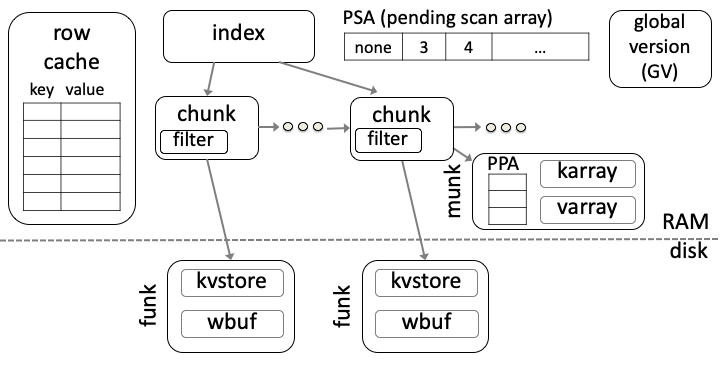
\includegraphics[width=0.9\columnwidth]{PiWi.png}
}
\caption{\sys\ data layout.}
\label{fig:layout}
\end{figure}

\paragraph{Chunk-based layout.}

\sys's data layout is depicted in Figure~\ref{fig:layout}.
Similarly to BTrees \Idit{and other disk-friendly data structures?}, 
\sys\ organizes data in fixed-size \emph{chunks}, each holding a contiguous key range.
This improves the efficiency of both disk access and memory access, in particular, for large range scans. 
At run-time, a list of all chunks is kept in RAM, where each chunk's data 
(consisting of keys in the corresponding range and values associated with them) 
is kept on disk (for persistence), and possibly in memory (for fast access). 

On disk, each chunk is associated with a \emph{file chunk}, or \emph{funk} --
a persistent data structure consisting of three files:  a value store \emph{vstore}, 
a compacted and sorted  key store \emph{kstore}, and a write buffer \emph{wbuf}. The vstore holds all the values associated with keys
in the chunk. When a funk is created, the kstore holds all the chunk's keys with pointers to corresponding values and the wbuf is empty.
New keys are subsequently appended to the unsorted wbuf, while new values are appended to the chunk's vstore.

This structure allows us to benefit from sorted searches on the kstore, and at the same time
allows for updating chunks without re-writing existing data, thus minimizing write amplification.
As a funk's wbuf grows, however, searching becomes inefficient   and  
the funk is no longer compact, i.e., it may contain redundant (over-written keys).
Therefore, once the wbuf exceeds a certain threshold, we reorganize the funk.

Since updates to disk are executed synchronously,  the data store reflecting all completed put operations 
can be consistently recovered from the on-disk funks at any time. \Idit{Need to discuss recovery somewhere.}

A subset of the chunks is also cached in memory to allow fast access, where each cached chunk is associated with a
\emph{memory chunk (munk)}  data structure. 
Munks are volatile and can be removed and recreated from funks at any time.
Thus, multiple \emph{generations} of munks may exist for a chunk throughout its life time.


At run-time, \sys\ holds in memory a linked list of chunk objects as well as 
%representing all funks in the data store. Chunks are also indexed in-memory for fast access by key using 
a \emph{chunk index}, which is a sorted map from keys to chunks (e.g., a sorted array, skip list, or search tree).
Note that since chunk objects do not hold actual keys and values, they are significantly smaller than munks and funks. 
\inred{A typical chunk object is smaller than 1KB, whereas the size of a funk or munk that holds 10K to 100K keys 
ranges between 1M to 100M depending on the data size. A typical \sys\ node holds thousands of chunks, with 
all chunk objects in memory in addition to hundreds of munks.} 


A munk consists of two arrays -- karray and varray -- where the karray implements a sorted linked list of the chunk's keys. 
When a munk is created, its karray is sorted by key, so each cell's successor in the linked list is the ensuing cell in the array.
As new keys are added, they create bypasses in the linked list and karray is no longer sorted.
Key removals, in turn, leave obsolete values in the karrray, so it is no longer compacted.

As key-value pairs are added, overwritten, and removed, munks and funks need to undergo reorganization. This includes  
\emph{compaction} to deallocate removed and overwritten data, 
\emph{sorting} keys to make searches more efficient,  and
\emph{splitting} overflowing chunks.
\remove{, and \emph{merging} under-utilized ones.}
All reorganizations are performed by \sys's \emph{rebalance} operation.
If the chunk has a munk, then rebalance compacts and sorts the munk in-memory by creating a new 
(compacted and sorted) munk instead of the existing one. 
Funks of uncached chunks are also compacted by replacing them with new funks, albeit less frequently.
Splits  create new chunks as well as new  funks (and possibly munks) associated with them.


\paragraph{Data structures.}

In addition to the chunk list and chunk index, \sys\ keeps a \emph{global version (GV)} for supporting atomic snapshot scans,
as described below; it tracks active scans in a \emph{pending scan array (PSA)} for garbage collection purposes (old 
versions not needed by any active scan can be reclaimed).

The chunk data structure is given in Algorithm~\ref{alg:chunk}. 
The first field is its status, which is explained  below. 
It next holds a pointer to the appropriate funk, and, if applicable, also munk, as well as a pointer to the next 
chunk in the chunk linked list.
It further keeps the generation number of its latest munk and a per-generation sequence number,
which, in case there is an active munk, is the index of the next free cell in the munk's karray and varray.


\begin{algorithm}[htb]
\begin{algorithmic}
\State status \Comment  baby, child, active, asleep, or aged
\State ptr funk \Comment funk disk address
\State ptr munk \Comment munk memory pointer
\State ptr next \Comment next chunk in linked list
\State int gen \Comment munk generation
\State int seq \Comment sequence number in current generation 
\State asymmetric lock rebalanceLock \Comment r/w lock 
\State lock funkChangeLock \Comment acquired with try\_lock 
\State PPA[threads] \Comment pending put array
\end{algorithmic}
\caption{Chunk data structure.}
\label{alg:chunk}
\end{algorithm}


The chunk additionally includes locks and data structures to synchronize concurrent access by multiple threads.
The replacement of a chunk (due to a split) or of a funk or munk associated with a given chunk 
must be executed atomically, and moreover, must be synchronized with concurrent puts. 
This is controlled by the chunk's rebalanceLock, which is held for short time periods
during chunk/funk/munk replacements.  It is a shared/exclusive lock (r/w lock), acquired in shared mode 
by put operations and in exclusive mode by rebalance. Gets and scans do not need to acquire the lock at all,
and are completely wait-free.

To minimize I/O, we allow at most one thread to rebalance a funk at a given time; this is controlled by 
the  funkChangeLock. This lock is used at a coarse granularity -- it is held throughout the creation of the new funk. 
It is acquired using a try\_lock call, and threads that fail to acquire it do not retry, but instead wait for the winning thread 
to complete the funk's creation.
Finally, the chunk holds a data structure called PPA for synchronizing  puts with concurrent scans, as explained in the next section. 


\subsection{Supporting atomic scans}
\label{ssec:scans}


\paragraph{Multi-versioning.}

We support atomic scans via multi-versioning using a system-wide global version, GV. 
A scan operation creates a \emph{snapshot} associated with GV's current value by incrementing GV, 
which signals to ensuing put operations that they must not overwrite values associated with 
smaller versions than the new GV value.
This resembles a \emph{copy-on-write (CoW)} approach, which virtually creates a snapshot by 
indicating that data pertaining to the snapshot should not be modified in place.  

To allow garbage collection of old versions, \sys\  maintains 
a pending scan array, PSA, with one entry per active thread, tracking snapshot times of ongoing scans.
The compaction process that runs as part of rebalance removes versions that are no longer required for any  
scan in the PSA. Specifically, for each key, it removes all but the last version that is smaller than the minimal
PSA entry. 

For linearizing (i.e., determining an order on) updates, we associate each key-value pair written to the data store 
with a unique-per-key identifier.
This identifier is a tuple $\langle$ver, gen, seq$\rangle$, where \emph{ver} is  the version read from GV 
(recall that GV is only incremented upon scans and hence might remain unchanged across multiple puts),
\emph{gen} is the generation of the target chunk's last created munk  (which may or may not still exist), 
and seq is the running sequence number of values inserted to the chunk in the current generation.

\paragraph{Concurrent puts and scans.}

A put operation obtains a version number from GV, and a scan begins by fetching and incrementing GV.
If a put obtains its version before a scan, then the new value must be included in the scan's snapshot. 
However, because the put's access to the GV and the insertion of the new value to the chunk do not occur atomically,
a subtle race may arise. Consider a put operation that obtains version $7$ from GV and then stalls before
inserting the value to the chunk, while a scan obtains version $7$ and increments GV to $8$. The scan then proceeds 
to read the appropriate chunk and does not find the new value although it should be included in its snapshot.

To remedy this, we rely on a mechanism previously proposed in~\cite{kiwi} for synchronizing puts and scans in an in-memory map.  
The idea is to have scans ``help'' puts obtain a version, and to make the inserted key-value pair visible the moment it has a version.
The per-chunk PPA is used to synchronize pending puts  with ongoing scans. 
The PPA holds an entry for every active inserting thread.
A put operation first registers itself in the appropriate chunk's PPA entry with the key and value it intends to add.
It thens reads GV, and attempts to set the version field in its PPA entry to the read version using an atomic 
compare-and-swap (CAS) instruction. A scan, in turn, scans the PPA in addition to the chunk's data (karray 
or kstore). If it finds a value associated with a version, it considers it to have been inserted (and returns it if the version is
the highest version for this key that does not exceed its scan time). If it encounters a value without a version, the scan helps the put
assign a version, also by attempting to CAS the PPA's version field to the current value of GV.
For symmetry, get operations synchronize with puts the same way that scans do. 

\subsection{Reorganization}
\label{ssec:rebalance}


\paragraph{Chunk life cycle.}

As a result of a rebalance operation, a chunk can undergo three types of changes: munk rebalance, funk rebalance,
(when a munk does not exist), and split. The latter affects the chunk object, the munk (if exists), and the funk.

In case of a munk rebalance, the chunk is immutable throughout the rebalance operation, and put operations targeting that chunk must
wait or help rebalance to complete. In this simple case, the chunk's status changes to \emph{asleep} -- indicating that it is immutable -- 
when rebalance begins, and changes back to \emph{active} when rebalance ends. 
\inred{Note that the asleep status is tantamount to the rebalanceLock being held in exclusive mode.}

Since funk rebalance involves I/O, it may take a long time, and so we  refrain from sleeping for its entire 
duration. Instead, we begin the funk creation in the background, when the chunk is still active, 
allowing new puts to proceed in wbuf. Once the new funk contains all the keys that were in the old one when 
rebalance started, we put the chunk to sleep,  
migrate the wbuf's new tail to the new chunk, swing the funk pointer in the chunk, and then make the chunk active again.


\begin{figure}[htb]
\centerline{
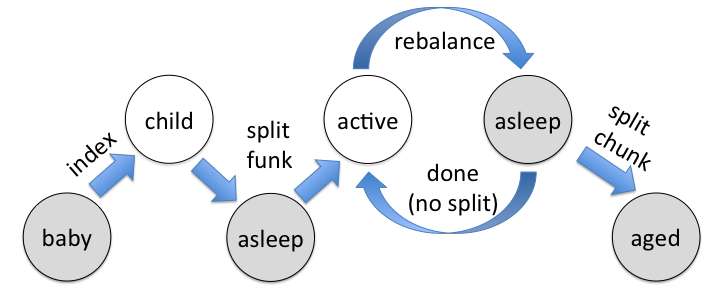
\includegraphics[width=\columnwidth]{state-diagram.png}
}
\caption{Chunk lifecycle; immutable states are grey and mutable ones are white.}
\label{fig:status}
\end{figure}

In the third case, the chunk is asleep when we create two new chunks to replace it. 
If the chunk has a munk, we split the munk (by creating two new munks) and update the appropriate pointers in the new chunks.  
Since creating new funks again involves I/O, we do not wish to keep the chunk immutable for the duration of this process,
and allow this process to proceed in the background while the two new chunks still point to the same old funk. 

After we replace the old chunk in the list with the two new ones, 
the old chunk is still accessible via the chunk index (even though it is no longer in the list). 
The new chunks are therefore created in \emph{baby} status, indicating that they are still immutable. 
Once the new chunks are indexed, the old chunk is \emph{aged}, and the new chunks can become mutable.
At this point, we change their status to \emph{child}, indicating that they are no longer immutable, but share a funk with another chunk,
which should be taken into account in future rebalances. Once the funk split completes, we put the chunk to sleep in order
to complete the funk switch and then change the chunk status  back to active. 
The chunk's life-cycle is depicted in Figure~\ref{fig:status}.



\paragraph{Synchronizing puts and rebalances.}


\subsection{\sys\ operations}
\label{ssec:ops}

\inred{Consider if we want full pseudocode}









